\chapter[RESULTADOS E CONCLUSÕES FINAIS]{RESULTADOS E CONCLUSÕES FINAIS} \label{concu:teo}

O acelerador de partículas LHC busca encontrar respostas sobre os fundamentos da matéria, mais especificamente as partículas físicas elementares. O estudo envolve uma enorme quantidade de dados e consequentemente uma enorme quantidade de colisões de partículas. Por conta dessa alta taxa de colisões, os sistemas eletrônicos desenvolvidos para o colisor trabalham em uma velocidade muito alta de processamento e estão imersos em um ambiente de uma taxa de radiação elevada. 

A transmissão de dados entre os dispositivos eletrônicos do LHC possui diversos problemas. Estes problemas referem-se à alta velocidade de processamento e a alta radiação que os dispositivos estão expostos. A alta velocidade  de processamento gera diversos problemas nas comunicações digitais, como por exemplo a dessincronização entre os dispositivos emissor e receptor. O ambiente com alta radiação induz ruídos nos dados transmitidos, sendo necessário um mecanismo de detecção de erros. O sistema implementado da codificação 64b66b possibilita a detecção de erros nos dados transmitidos e o sincronismo entre os dispositivos comunicantes. A detecção de erros na codificação 64b66b não é robusta, sendo necessário implementar um CRC. Dependendo da característica deste sistema pode-se detectar todos os erros inseridos na transmissão. O sincronismo é garantido por meio do \textit{scrambler}, uma vez que esse sistema fornece um balanço no número de bits $1's$ e $0's$ sendo possível circuitos recuperadores de \textit{clock} atuarem.

O estudo das características da codificação 64b66b foi obtido testando o sistema descrito no programa Matlab\textsuperscript{TM}, dentro do ambiente do Simulink. O programa desenvolvido da codificação recebe os 64 bits na entrada do sistema passando-o pelo CRC, posteriormente pelo \textit{scrambler} e no final adiciona os 2 bits de sincronismo. Posteriormente o dado codificado de 74 bits passa pelo canal de transmissão que pode ser adicionado erros ou não. O sistema da decodificação do dado de 74 bits possui o caminho inverso. Primeiramente o dado sem os bits de sincronismo passa pelo \textit{descrambler} desembaralhando o dado. Este dado desembaralhado é inserido no CRC para verificar se ocorreram erros. Posteriormente, faz-se uma verificação dos registradores do CRC (se estão todos em nível lógico $0$) e os bits de sincronismo (se são $'01'$). Caso contrário é fornecido um sinal de erro no \textit{decoder}. 

Para uma simulação de teste, introduziu-se no BBG uma probabilidade de erro de 40\% e obteve-se o número de erro introduzidos, detectados e também os gerados pelo \textit{scrambler}. Esta simulação está descrita na \autoref{simulacaoSys} e no total foram transmitidos 10000 pacotes de 74 bits.

\begin{figure}[H]
	\caption{\label{simulacaoSys} Simulação do sistema implementado da codificação 64b66b.}
	\centering
	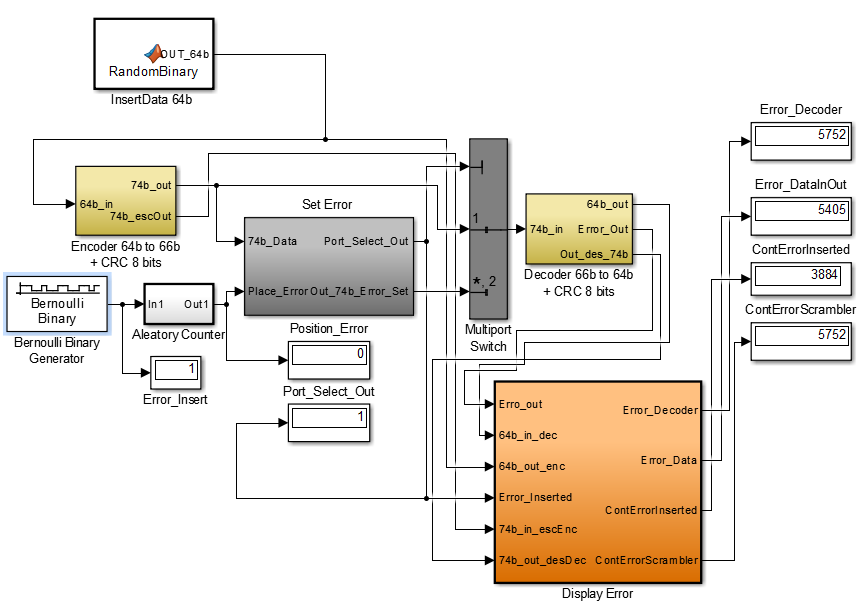
\includegraphics[scale=0.7]{systemTest.png}
	\begin{center}
		Fonte: Elaborado pelo Autor
	\end{center}	
\end{figure}

Para uma probabilidade de erro no canal de 40\%, obteve-se 3884 erros inseridos presentes no \textit{display} $ContErrorInserted$ e 5752 erros gerados ao total obtidos pelo \textit{display} $ContErrorScrambler$. Pode-se observar o comportamento do \textit{scrambler} na presença de erros, uma vez que o número de erros presentes na transmissão é maior do que o número de erros inseridos no canal. Isto deve-se ao fato de o \textit{descrambler} carregar um erro para o novo dado de entrada em alguns casos. Estas possibilidades foram descritas na \autoref{scramb:64b66b}. 

Pelo \textit{display} $Error\_Decoder$ obteve-se 5752 erros detectados, sendo o mesmo número de erros gerados após o \textit{descrambler} atuar no dado transmitido. Desta forma, pode-se confirmar a teoria desenvolvida no \autoref{crc:teoria} uma vez que o CRC detectou todos os erros únicos gerados no sistema. Portanto, o sistema desenvolvido para detectar erros é bastante confiável e robusto, capaz de fornecer dados totalmente confiáveis ao final da decodificação pois sinaliza os que estão errados para erros únicos.

Pelo \textit{display} $Error\_dataInOut$ obteve-se 5405 erros detectados entre o dado de entrada e o de saída de 64 bits, sendo menor que o total de erros detectados no \textit{decoder}. Isto acontece pois o erro pode ocorrer dentro da faixa do dado de 64 bits, dos 2 bits de sincronismo ou do resultado de 8 bits do CRC. Desta forma, o número de erros entre o dado de entrada e de saída do sistema da codificação é explicado pelo fato de algumas vezes o erro ocorrer na faixa do dado do CRC ou dos bits de sincronismo.

Em uma transmissão de dados em alta velocidade é impossível não haver erros na transmissão, mesmo com a implementação de uma codificação muito robusta. Nota-se que o sistema cumpre as características da codificação, pois ao codificar obtêm-se dados para serem transmitidos com a quantidade de bits 0’s e bits 1’s balanceada garantidos pelo sistema \textit{scrambler}. No lado do \textit{decoder} é possível detectar todos os erros na transmissão por meio do CRC implementado.  

Para observar a proporção de erros em relação ao número de dados transmitidos no sistema, configurou-se no ambiente Simulink o número máximo de simulações para $1000$ com passos de $0.1$ totalizando $10000$ simulações. Variou-se a probabilidade de erro no canal no bloco \textit{Bernoulli Binary Generator} de $0$ até $40$ por cento, coletando o número de erros da comparação entre o dado de entrada e saída do sistema ($Error\_DataInOut$), de entrada e saída do \textit{scrambler} ($ContErrorScrambler$), do sinal de erro do \textit{decoder} ($Error\_Decoder$) e o número de erros inseridos no sistema ($ContErrorInserted$). Na \autoref{test_data}, observa-se a porcentagem de erro obtido na transmissão de acordo com a variação da probabilidade de erro no canal.

\begin{table}[htb]
	\ABNTEXfontereduzida
	\caption[Tabela de dados da simulação]{Porcentagem de erros obtidos com a variação da probabilidade de erro no canal do sistema da codificação 64b66b}
	\label{test_data}
	\begin{tabular}{ >{\centering\arraybackslash}m{2.75cm} | >{\centering\arraybackslash}m{2.75cm} | >{\centering\arraybackslash}m{2.75cm} | >{\centering\arraybackslash}m{2.75cm} | >{\centering\arraybackslash}m{2.75cm} }
		\hline
		\centering \textbf{Probabilidade de erro no Canal(\%)} & \textbf{Erro detectado pelo decoder(\%)} & \textbf{Erro no dado de entrada e saída de 64 bits(\%)} & \textbf{Erros Inseridos no canal de transmissão(\%)} & \textbf{Erro no dado de entrada e saída do scrambler(\%)}\\
		\hline
		\textbf{0} & 0 & 0 & 0 & 0\\
		\hline
		\textbf{1} & 1,52 & 1,34 & 0,9 & 1,52\\
		\hline
		\textbf{2} & 3,14 & 2,82 & 1,81 & 3,14\\
		\hline
		\textbf{3} & 4,77 & 4,34 & 2,74 & 4,77\\
		\hline
		\textbf{4} & 6,44 & 5,85 & 3,66 & 6,44\\
		\hline
		\textbf{5} & 8,38 & 7,65 & 4,87 & 8,38\\
		\hline
		\textbf{6} & 10,19 & 9,33 & 5,91 & 10,19 \\
		\hline
		\textbf{7} & 11,73 & 10,74 & 6,87 & 11,73\\
		\hline
		\textbf{8} & 13,19 & 12,04 & 7,76 & 13,19\\
		\hline
		\textbf{9} & 14,90 & 13,60 & 8,75 & 14,9\\
		\hline
		\textbf{10} & 16,35 & 14,95	& 9,63 & 16,35\\
		\hline
		\textbf{11} & 17,92 & 16,38 & 10,59 & 17,92\\
		\hline
		\textbf{12} & 19,32 & 17,70 & 11,52 & 19,32\\
		\hline
		\textbf{13} & 20,53 & 18,87 & 12,31 & 20,53\\
		\hline
		\textbf{14} & 22,23 & 20,44 & 13,40 & 22,23\\
		\hline
		\textbf{15} & 23,73 & 21,85 & 14,30 & 23,73\\
		\hline
		\textbf{16} & 25,12 & 23,16 & 15,20 & 25,12\\
		\hline
		\textbf{17} & 26,98 & 24,85 & 16,37 & 26,98\\
		\hline
		\textbf{18} & 28,85 & 26,59 & 17,57 & 28,85\\
		\hline
		\textbf{19} & 30,32 & 28,04 & 18,58 & 30,32\\
		\hline
		\textbf{20} & 31,66 & 29,34 & 19,46 & 31,66\\
		\hline
		\textbf{21} & 33,23 & 30,82 & 20,52 & 33,23\\
		\hline
		\textbf{22} & 34,45 & 32,03 & 21,41 & 34,45\\
		\hline
		\textbf{23} & 35,81 & 33,26 & 22,35 & 35,81\\
		\hline
		\textbf{24} & 37,05 & 34,42 & 23,29 & 37,05\\
		\hline
		\textbf{25} & 38,66 & 35,89 & 24,40 & 38,66\\
		\hline
		\textbf{26} & 39,93 & 37,06 & 25,31 & 39,93\\
		\hline
		\textbf{27} & 41,33 & 38,40 & 26,31 & 41,33\\
		\hline
		\textbf{28} & 42,73 & 39,74 & 27,36 & 42,73\\
		\hline
		\textbf{29} & 44,14 & 41,09 & 28,40 & 44,14\\
		\hline
		\textbf{30} & 45,50 & 42,39 & 29,36 & 45,50\\
		\hline
		\textbf{31} & 47,07 & 43,89 & 30,45 & 47,07\\
		\hline
		\textbf{32} & 48,29 & 45,10 & 31,40 & 48,29\\
		\hline
		\textbf{33} & 49,45 & 46,25 & 32,30 & 49,45\\
		\hline
		\textbf{34} & 50,59 & 47,36 & 33,17 & 50,59\\
		\hline
		\textbf{35} & 51,88 & 48,56 & 34,16 & 51,88\\
		\hline
		\textbf{36} & 53,14 & 49,78 & 35,18 & 53,14\\
		\hline
		\textbf{37} & 54,21 & 50,86 & 36,16 & 54,21\\
		\hline
		\textbf{38} & 55,14 & 51,78 & 36,99 & 55,14\\
		\hline
		\textbf{39} & 56,36 & 52,97 & 37,93 & 56,36\\
		\hline
		\textbf{40} & 57,52 & 54,05 & 38,84 & 57,52\\
		\hline
	\end{tabular}
	\begin{center}
		Fonte: Elaborada pelo autor.\
	\end{center}
\end{table}

Na \autoref{plotdata} é apresentado um gráfico com os dados da \autoref{test_data}. Observa-se que o comportamento da codificação em relação aos erros acometidos em um bit do dado transmitido, é aproximadamente linear para todas as probabilidades de erro no canal até 40\%. Pelos dados observados, o \textit{decoder} é capaz de detectar todos os erros gerados no canal. Observa-se, que a diferença entre os erros do dado de entrada e saída do \textit{scrambler} e o erro inserido no canal é no máximo de aproximadamente 20\%, de acordo com a simulação de até 40\% de probabilidade de erro no canal. Em casos de baixa probabilidade de erro no canal de transmissão, a diferença está em torno de 10\%. Dessa forma, observa-se que a codificação é adequada para a transmissão uma vez que mesmo gerando mais erros do que os inseridos é possível identificá-los em sua totalidade.

\begin{figure}[H]
	\caption{\label{plotdata} Gráfico do comportamento da codificação 64b66b em relação aos erros.}
	\centering
	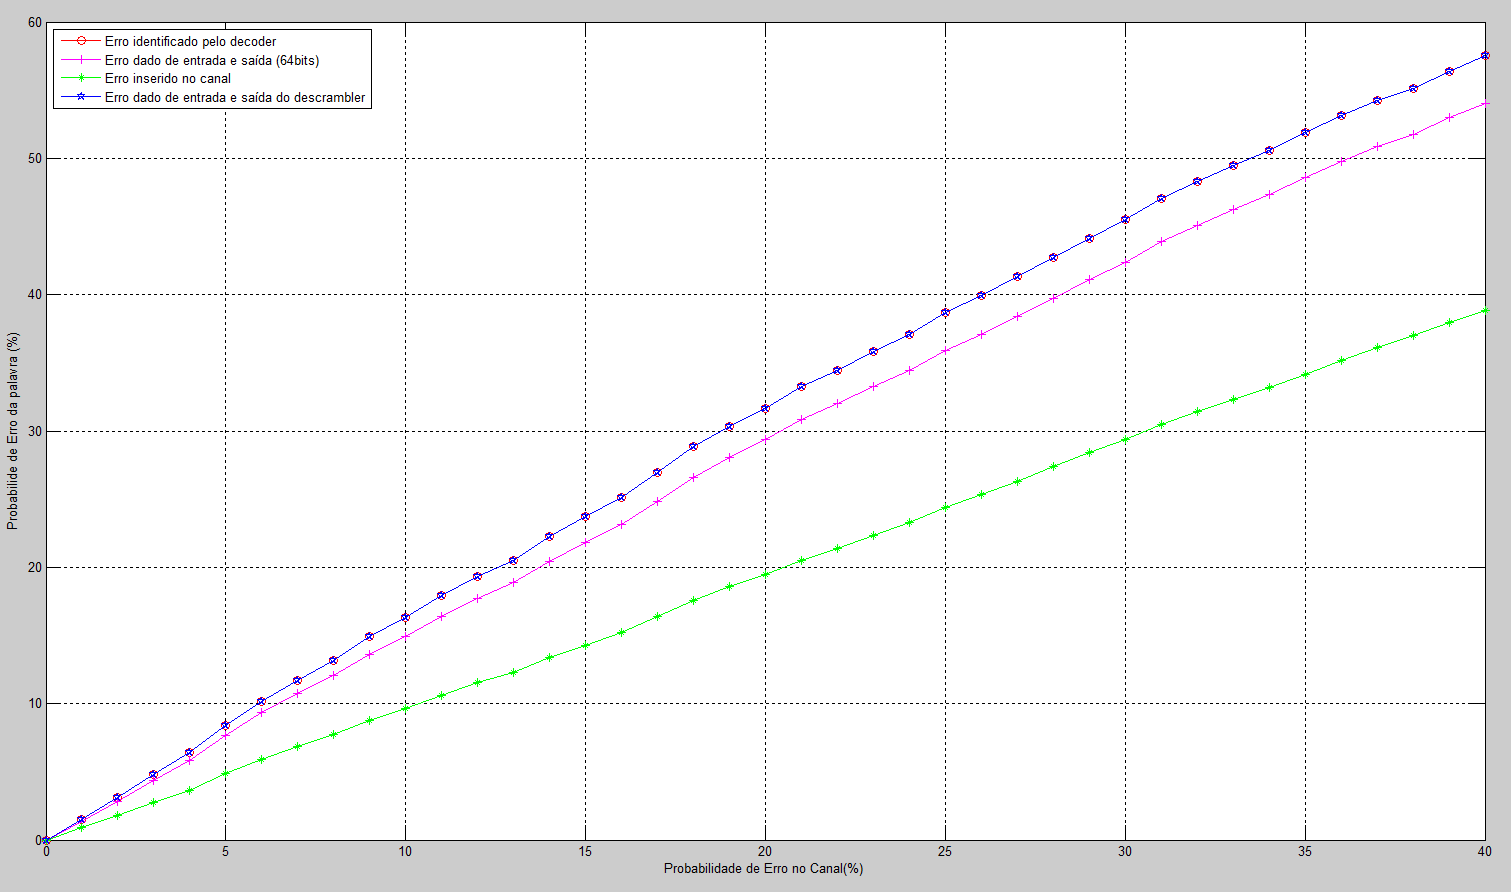
\includegraphics[scale=0.4]{plotdata_system64b66b.png}
	\begin{center}
		Fonte: Elaborado pelo Autor
	\end{center}	
\end{figure}

Para transmissões em alta velocidade, normalmente trabalha-se com uma probabilidade de erro de aproximadamente 5\% no canal de transmissão. Na \autoref{plotdata20} é apresentado o gráfico com os dados da \autoref{test_data} traçados com uma probabilidade de erro no canal de transmissão de até 20\%. Neste caso, observa-se um comportamento aproximadamente linear, sendo obtido uma porcentagem de erro no dado de entrada e saída do \textit{scrambler} de 8.38\% para uma probabilidade de erro no canal de 5\% , de acordo com a \autoref{test_data}. Para uma probabilidade de erro no canal de 5\%, o \textit{decoder} identificou todos os erros gerados, dessa forma a porcentagem de erro na transmissão pode ser reduzida a zero.

\begin{figure}[H]
	\caption{\label{plotdata20} Comportamento do sistema da codificação 64b66b com a probabilidade de erros de até 20\%.}
	\centering
	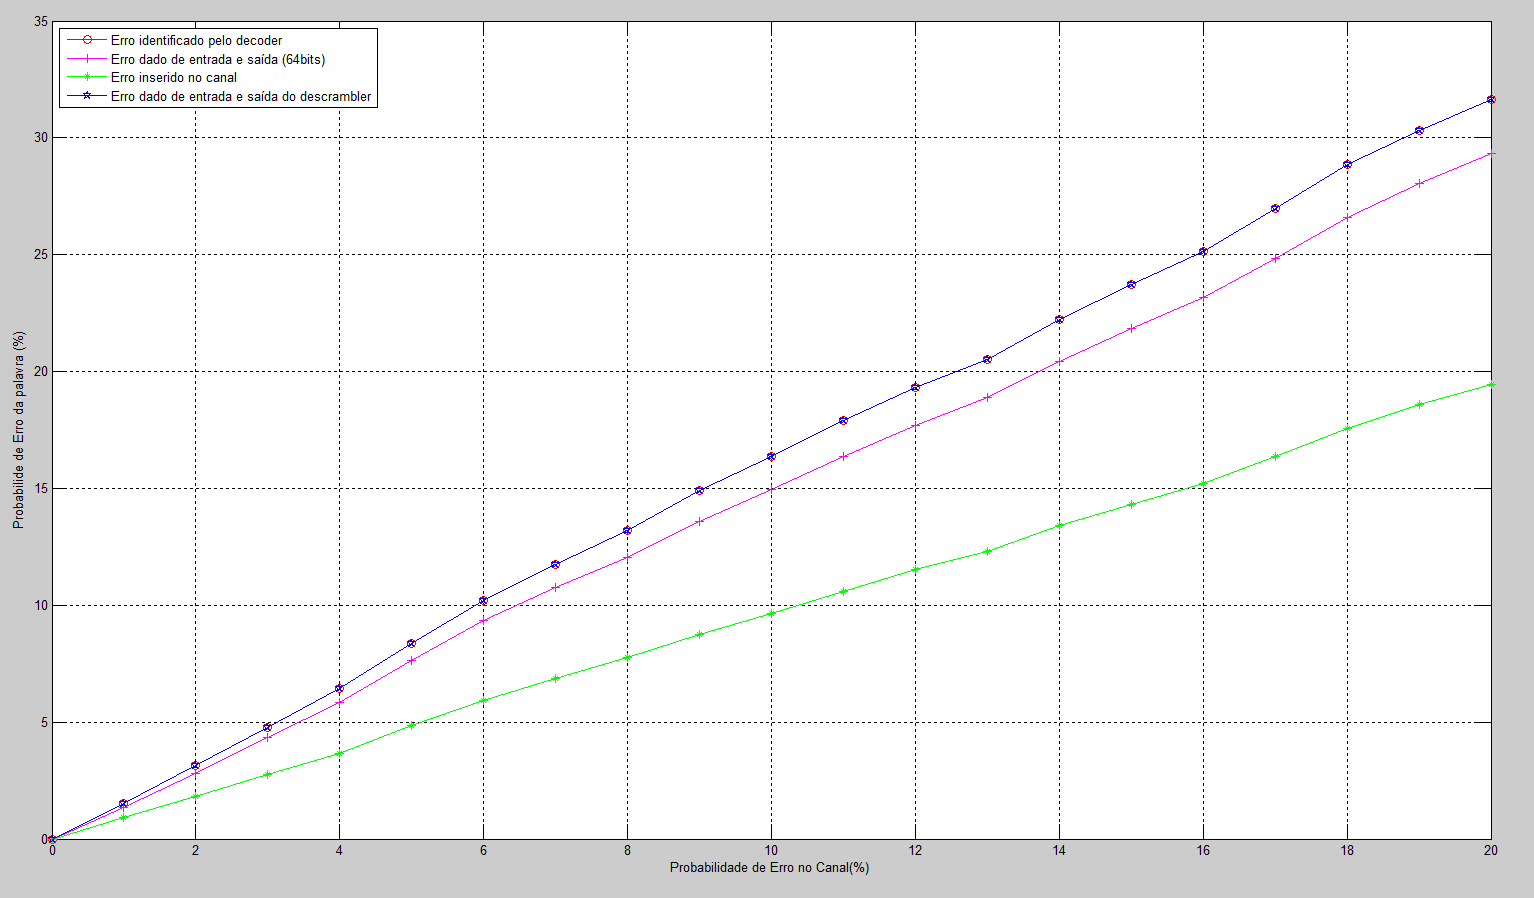
\includegraphics[scale=0.4]{plotdata20_system64b66b.png}
	\begin{center}
		Fonte: Elaborado pelo Autor
	\end{center}	
\end{figure}

Tanto o sistema do \textit{encoder} e \textit{decoder}, foram intensamente testados e analisados por meio das entradas e saídas produzidas, observando a capacidade de detecção de erros e a taxa de erros adicionais inserido no sistema por meio do \textit{scrambler}. Observou-se que o sistema descrito no software Matlab\textsuperscript{TM} no ambiente do Simulink é capaz de codificar e decodificar dados seguindo a descrição da codificação 64b66b, além de ser capaz de identificar todos os erros simples gerados no canal de transmissão por meio do CRC implementado. 

As características obtidas da codificação, observou-se que o sistema implementado gera um \textit{overhead} na palavra codificada total de 15,625\%, contra os 3,125\% descritos pela codificação original. Este aumento no \textit{overhead} da palavra codificada deve-se à introdução do CRC 8 bits introduzido para detecção de erros, uma vez que a descrição da codificação 64b66b não possui uma detecção de erros robusta. Porém, um \textit{overhead} de 15,625\% é menor do que 25\% descritos pela codificação 8b10b. 

Portanto, conclui-se que uma implementação em um sistema real pode definir qual a melhor codificação a ser utilizada para um ambiente de transmissões de dados puros em alta velocidade. Este tipo de comparação é necessária uma vez que em uma implementação real em um FPGA deve-se considerar outros fatores, como por exemplo o \textit{delay} na codificação do dado.
